\section{Série de Mercator}

Ainda no espectro da matemática, após a descoberta da íntima conexão entre a função logaritmo e área sobre a hipérbole começaram a surgir consequências da propriedade. 

A Série de Mercator é um dos principais marcos. Inicialmente, a série foi descoberta independemente por Johannes Hudde (1656) e por Isaac Newton (1665), entretanto, nenhum dos dois havia publicado o resultado. Apenas em 1668, Nicholas Mercator após descobrir de forma independente publicou o seu tratado Logarithmotechnia com a seguinte série:

\begin{equation*}
    \ln(1+x) = x - \dfrac{x^2}{2} + \dfrac{x^3}{3} - \dfrac{x^4}{4} + \ldots
\end{equation*}

que aproxima a função logaritmo para o intervalo $-1<x \le 1$.

\subsection{Demonstração}

Note que a propriedade de a área da hipérbole se relacionar ao logaritmo pode ser resumida em: 
\begin{equation}
    \ln(1+x) = \int_{0}^{x}\dfrac{1}{1+t}dt
\end{equation}


Na época de Mercator, as séries geométricas já eram difundidas, daí os matemáticos da época já conheciam a seguinte expressão:

\begin{equation} \label{eq:serie_geo}
    \frac{1}{1-x} = 1 + x+x^2+x^3 + \ldots
\end{equation}

Ao analisar a expressão dentro da integral, Mercator percebeu que a expressão (\ref{eq:serie_geo}) ao tomar $x = -t$ se torna:

\begin{equation}
    \dfrac{1}{1+t} = 1 -t+t^2-t^3 + \ldots
\end{equation}

Daí:

\begin{equation}
    \ln(1+x) = \int_{0}^{x}\dfrac{1}{1+t}dt = \int_{0}^{x} 1 -t+t^2-t^3 + \ldots dt
\end{equation}


Como a integral em (4) é polinomial, é facil calcular a primitiva:

\begin{align*}
    \int_{0}^{x} (1 -t+t^2-t^3 + \ldots) \,dt &= \left[ t - \frac{t^2}{2} + \frac{t^3}{3} - \frac{t^4}{4} + \ldots \right]_{0}^{x} \\
                                              &= x - \frac{x^2}{2} + \frac{x^3}{3} - \frac{x^4}{4} + \ldots
\end{align*}

Note que, o resultado nada mais é do que um caso específico da Série de Taylor com $f(x) = \ln(1+x)$ em $x=0$.

\begin{equation*}
    f(x) = \sum_{n=0}^{\infty} a_n (x-a)^n \qquad \text{sendo} \qquad a_n = \frac{f^{(n)}(a)}{n!}
\end{equation*}

Ao calcular as derivadas consecutivas:
\begin{align*}
    f(x) &= \ln(1+x) \\
    f'(x) &= \frac{1}{1+x} \\
    f''(x) &= -\frac{1}{(1+x)^2} \\
    f^{(3)}(x) &= \frac{2}{(1+x)^3} \\
    f^{(4)}(x) &= -\frac{6}{(1+x)^4} \\
    &\vdots
\end{align*}

Agora, avaliamos tudo em $x=0$:

\[
f(0) = 0, \quad f'(0) = 1, \quad f''(0) = -1, \quad f^{(3)}(0) = 2, \quad f^{(4)}(0) = -6, \ldots
\]

Por fim, substituindo:
\begin{align*}
    \ln(1+x) &= f(0) + f'(0)x + \frac{f''(0)}{2!}x^2 + \frac{f^{(3)}(0)}{3!}x^3 + \frac{f^{(4)}(0)}{4!}x^4 + \ldots \\
             &= 0 + 1x + \frac{-1}{2}x^2 + \frac{2}{6}x^3 + \frac{-6}{24}x^4 + \ldots
\end{align*}

Ao simplificar, novamente obtemos a Série de Mercator:

\[
\ln(1+x) = x - \frac{x^2}{2} + \frac{x^3}{3} - \frac{x^4}{4} + \ldots
\]

\subsection{Gráfico}

\begin{figure}[H]
    \centering
    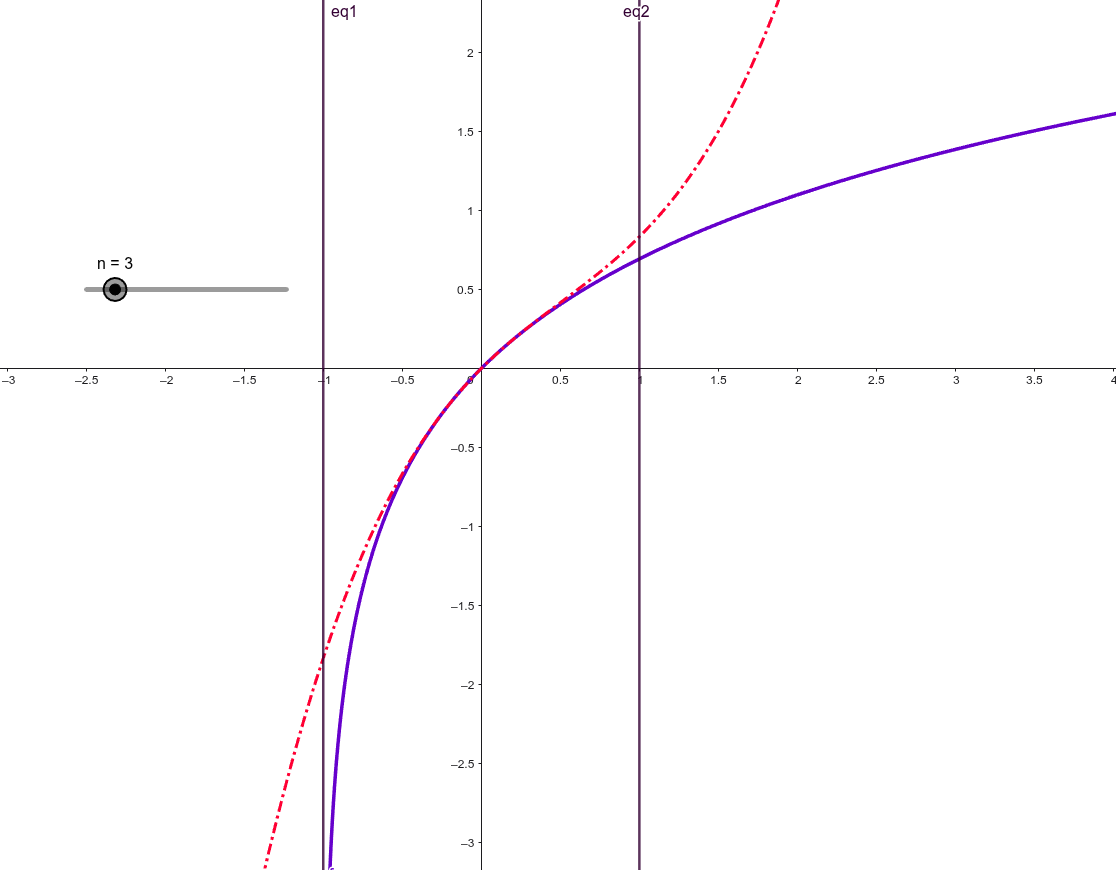
\includegraphics[width=\linewidth]{img/image.png}
    \caption{Comparação da Série de Mercator para $n=3$ e a função $\ln (1+x)$.}
\end{figure}

No GeoGebra, criamos um gráfico animado iterativo para enxergar como a Série de Mercator se aproxima da função $\ln (1+x)$ para $-1< x \le 1$ quando o número de iterações aumenta. Segue o link: 
\href{https://www.geogebra.org/calculator/jyycuaxp}{Clique Aqui}
